\chapter{Conceptos Teóricos}
\label{chap:conceptos}

Para comprender las decisiones de diseño y la implementación de la infraestructura de este TFG, es necesario primero asentar las bases teóricas sobre las que se construyen las tecnologías seleccionadas. Este capítulo profundiza en los paradigmas y arquitecturas clave del procesamiento de datos distribuidos, el streaming de vídeo y los conceptos de red y seguridad que son el núcleo de este proyecto.

\section{Paradigmas de Arquitecturas Distribuidas}
\label{sec:conceptos_arquitecturas}
Un sistema distribuido se compone de múltiples componentes de software autónomos, ejecutándose en diferentes nodos, que se comunican y coordinan entre sí para cumplir un objetivo común. El diseño de este tipo de sistemas se basa en una serie de patrones y paradigmas que garantizan su eficiencia, escalabilidad y tolerancia a fallos.

\subsection{Sistemas de Mensajería: El Modelo Publicar-Suscribir}
El modelo de comunicación Publicar-Suscribir (o \textit{Pub-Sub}) es un patrón de mensajería asíncrono donde las aplicaciones que envían mensajes, llamadas \textbf{productores} (\textit{publishers}), no los envían directamente a los receptores. En su lugar, los publican en canales o categorías lógicas, conocidas como \textbf{tópicos} (\textit{topics}), gestionados por un intermediario o \textit{broker}. Por otro lado, las aplicaciones que reciben los mensajes, llamadas \textbf{consumidores} (\textit{subscribers}), se suscriben a los tópicos de su interés para recibir los mensajes que se publican en ellos \cite{birman2007guide}.

La principal ventaja de este patrón es el \textbf{desacoplamiento} que introduce entre los componentes. Los productores no necesitan conocer a los consumidores, y viceversa. Esto permite que los sistemas escalen de forma independiente y que nuevos componentes puedan añadirse a la arquitectura sin necesidad de modificar los existentes, dota a la arquitectura de una enorme flexibilidad y escalabilidad \cite{kleppmann2017designing}.

\subsection{Virtualización a Nivel de Sistema Operativo}
La virtualización es una técnica que permite crear versiones virtuales de recursos informáticos. Mientras que las máquinas virtuales tradicionales emulan un sistema de hardware completo sobre el que se ejecuta un sistema operativo invitado, la \textbf{virtualización a nivel de sistema operativo}, más conocida como contenerización, sigue un enfoque diferente.

Los contenedores se ejecutan sobre el kernel del sistema operativo anfitrión, pero en espacios de usuario aislados. Cada contenedor tiene su propio sistema de ficheros, procesos y configuración de red, pero comparte el mismo kernel subyacente. Esto los hace extremadamente ligeros, rápidos de iniciar y mucho más eficientes en el uso de recursos que las máquinas virtuales, convirtiéndolos en la tecnología ideal para desplegar arquitecturas de microservicios.

\section{Fundamentos de Tecnologías de Streaming}
\label{sec:conceptos_streaming}

\subsection{El Log de Transacciones Distribuido e Inmutable}
Una de las arquitecturas más potentes para construir sistemas de mensajería y plataformas de \textit{streaming} de datos es el \textbf{log de transacciones distribuido} (o \textit{commit log}). Conceptualmente, es una estructura de datos inmutable a la que solo se pueden añadir registros. Una vez escrito, un registro no puede ser modificado ni eliminado.

En un sistema distribuido, este log se divide en \textbf{particiones} para permitir el paralelismo y la escalabilidad. Cada partición es un log ordenado que se replica a través de múltiples servidores (\textbf{brokers}) para garantizar la tolerancia a fallos y la alta disponibilidad. Cada registro en una partición tiene un identificador secuencial único llamado \textbf{offset}, que permite a los consumidores llevar un control preciso de su posición de lectura, incluso en caso de fallos. Este modelo es la base de sistemas de mensajería de alto rendimiento capaces de procesar millones de eventos por segundo.

\subsection{Modelo de Computación Distribuida en Memoria}
El procesamiento de grandes volúmenes de datos (\textit{Big Data}) requiere modelos de computación que puedan paralelizar el trabajo a través de un clúster de máquinas. La abstracción fundamental en los motores de procesamiento modernos es el \textbf{Conjunto de Datos Distribuido y Resiliente} (\textit{Resilient Distributed Dataset} o RDD). Un RDD es una colección de elementos inmutable y tolerante a fallos que puede ser procesada en paralelo \cite{zaharia2012resilient}.

Las operaciones sobre estos datos se dividen en:
\begin{itemize}
    \item \textbf{Transformaciones:} Operaciones que crean un nuevo conjunto de datos a partir de uno existente (ej. un filtrado). Son "perezosas" (\textit{lazy}), es decir, su cómputo no se realiza al momento.
    \item \textbf{Acciones:} Operaciones que disparan la ejecución de las transformaciones y devuelven un resultado o escriben en un sistema externo.
\end{itemize}
Cuando se invoca una acción, el motor de procesamiento analiza la cadena de transformaciones y construye un \textbf{Grafo Acíclico Dirigido (DAG)} de las operaciones. Este grafo es optimizado y dividido en etapas de tareas que se distribuyen entre los nodos del clúster para su ejecución paralela, permitiendo un procesamiento masivo y eficiente.

\subsection{Transmisión de Vídeo sobre IP}
La transmisión de vídeo en tiempo real a través de redes IP se basa en protocolos diseñados para manejar datos multimedia con baja latencia. Uno de los protocolos más extendidos para este fin es el \textbf{Protocolo de Mensajería en Tiempo Real (RTMP)}. Desarrollado originalmente para Adobe Flash, RTMP es un protocolo basado en TCP que mantiene una sesión persistente entre cliente y servidor, permitiendo la transmisión fiable de flujos de audio, vídeo y datos.

\section{Conceptos de Seguridad en Comunicaciones Web}
\subsection{HTTP, HTTPS y el Protocolo SSL/TLS}
HTTP (Hypertext Transfer Protocol) es el protocolo fundamental de la web, pero transmite la información en texto plano. \textbf{HTTPS} es su versión segura, que añade una capa de cifrado mediante el protocolo \textbf{SSL/TLS} (Secure Sockets Layer/Transport Layer Security) \cite{rescorla2001ssl}. Esta capa utiliza criptografía de clave pública para establecer una conexión segura, garantizando la confidencialidad (nadie puede leer la comunicación) y la integridad (nadie puede modificarla) de los datos.

\begin{figure}[H]
    \centering
    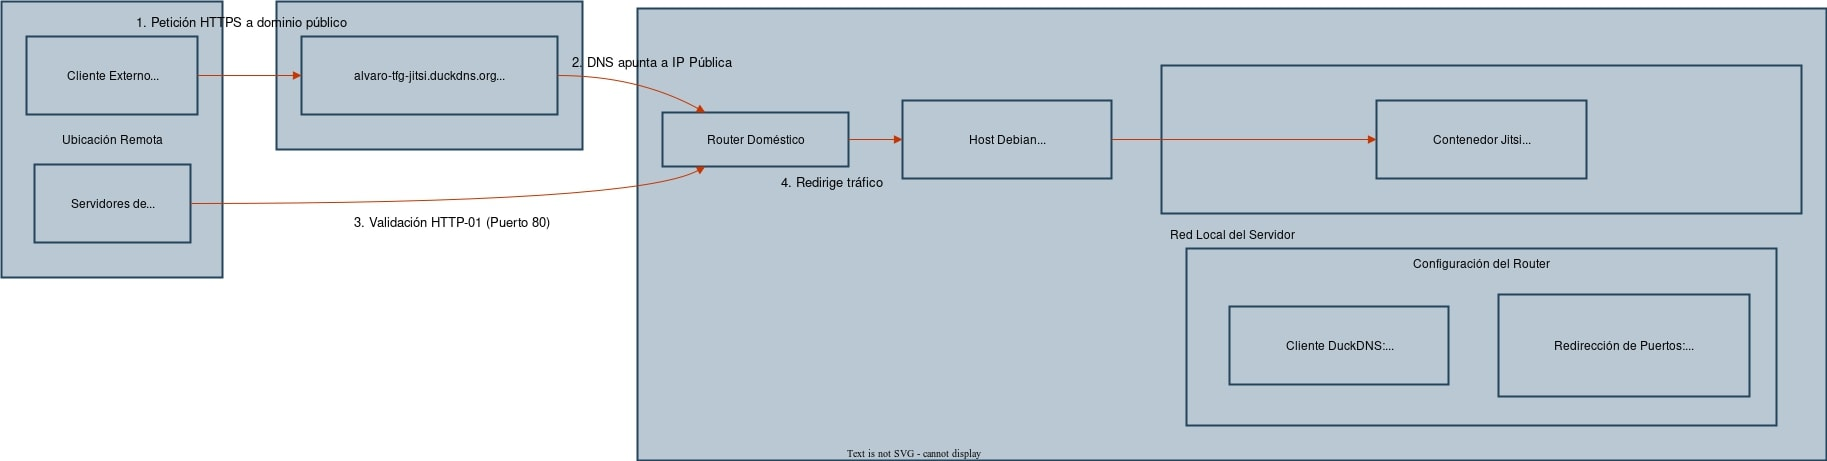
\includegraphics[width=0.9\textwidth]{img/ArquitecturadeRedparaelDesplieguedeJitsi.jpg}
    \caption{Arquitectura de red implementada para permitir el acceso externo seguro vía HTTPS y la validación de certificados de Let's Encrypt.}
    \label{fig:arquitectura_red_letsencrypt}
\end{figure}

\subsection{Certificados Digitales y Autoridades de Certificación}
Para que HTTPS funcione, el servidor debe presentar un \textbf{certificado digital SSL/TLS} que valide su identidad. Existen dos tipos principales:
\begin{itemize}
    \item \textbf{Certificados Autofirmados:} Son generados por el propio administrador del servidor. No son emitidos por una entidad de confianza, por lo que los navegadores web los rechazan por defecto, mostrando advertencias de seguridad al usuario.
    \item \textbf{Certificados de una CA:} Son emitidos por una \textbf{Autoridad de Certificación (CA)}, una entidad externa en la que confían los navegadores (como Let's Encrypt). Cuando un navegador recibe un certificado emitido por una CA de confianza, establece la conexión segura sin advertencias. Por motivos de seguridad, los navegadores modernos exigen una conexión HTTPS con un certificado válido para permitir el acceso a funcionalidades sensibles como la cámara o el micrófono.
\end{itemize}

\section{Componentes Conceptuales de un Pipeline de Datos}
\label{sec:conceptos_pipeline}
Toda arquitectura de procesamiento de datos, como la que se aborda en este proyecto, puede descomponerse en una serie de componentes lógicos, cada uno con una responsabilidad bien definida. La comprensión de estos roles es fundamental para diseñar un sistema robusto y escalable.
\begin{figure}[H]
    \centering
    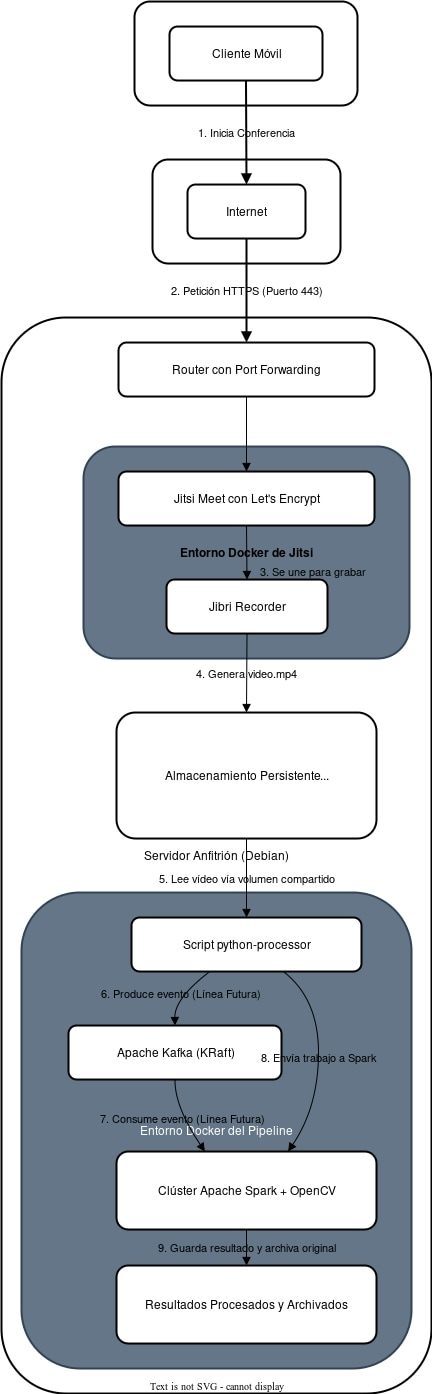
\includegraphics[height=0.9\textheight]{img/arquitectura-general.jpg}
    \caption{Visión general de la arquitectura del sistema, mostrando la interacción entre el subsistema de captura (Jitsi) y el pipeline de procesamiento (Kafka/Spark).}
    \label{fig:arquitectura_completa}
\end{figure}

\subsection{El Productor de Eventos (\textit{Producer})}
El \textbf{Productor} es cualquier entidad del sistema cuya función principal es originar o capturar datos y enviarlos a un sistema de mensajería. Este componente actúa como la fuente de información del pipeline. En el contexto de un sistema de análisis de vídeo, el rol del productor sería desempeñado por el sistema de captura, encargado de digitalizar la sesión y publicarla como un evento o una serie de eventos en el flujo de datos.

\subsection{El Intermediario de Mensajería (\textit{Broker})}
El \textbf{Broker} es el servidor o conjunto de servidores que forman el núcleo del sistema de mensajería. Su responsabilidad es recibir los eventos de los productores, almacenarlos de forma duradera y fiable, y ponerlos a disposición de los consumidores. En arquitecturas distribuidas, se despliega un clúster de brokers para garantizar la alta disponibilidad y la tolerancia a fallos. Este componente es esencial para desacoplar a los productores de los consumidores, permitiendo que operen a ritmos diferentes y de forma independiente.

\subsection{El Consumidor y Procesador de Datos (\textit{Consumer}/\textit{Processor})}
El \textbf{Consumidor} es la aplicación que se suscribe al sistema de mensajería para recibir y leer los eventos que le interesan. Una vez que un consumidor recibe un evento, se lo entrega a una lógica de \textbf{Procesamiento}, que es donde reside la inteligencia de la aplicación. Esta lógica es la que se encarga de transformar, analizar o actuar sobre los datos recibidos. En un sistema de procesamiento de vídeo, el consumidor se encargaría de recibir los datos del vídeo, y el procesador aplicaría los algoritmos de visión artificial sobre ellos.

\subsection{El Modelo de Computación Maestro-Trabajador (\textit{Master-Worker})}
Para procesar grandes volúmenes de datos de manera eficiente, los \textit{frameworks} de computación distribuida suelen emplear el patrón arquitectónico \textbf{Maestro-Trabajador} (conocido también como \textit{Driver-Executor}).
\begin{itemize}
    \item El nodo \textbf{Maestro} (\textit{Master} o \textit{Driver}) es el cerebro de la operación. Recibe el trabajo a realizar, lo divide en un conjunto de tareas más pequeñas e independientes, y las distribuye entre los nodos trabajadores. También se encarga de coordinar la ejecución y agregar los resultados finales.
    \item Los nodos \textbf{Trabajadores} (\textit{Workers} o \textit{Executors}) son los que realizan el trabajo pesado. Cada trabajador recibe una o más tareas del maestro, las ejecuta en paralelo con otros trabajadores sobre una porción de los datos, y devuelve el resultado al maestro.
\end{itemize}